\chapter{流形上的微积分}
\label{chap:manifold-calculus}

一元微积分基本定理说，函数导数在区间上的积分等于端点值之差；多元微积分中的Green、Gauss与Stokes公式说，区域内部某种导数的积分等于边界上的环流或通量。这些等式都写在欧氏坐标里。到了球面、环面或一般流形上，我们仍想问同样的问题：怎样对一个量求导，怎样在弯曲的区域上积分，内部的变化怎样汇总到边界。回答之前要先说清楚，被求导、被积分的对象是什么，每项运算需要哪些结构。

本章分两步展开。第一步只用光滑结构。第~\ref{sec:mcalc-forms}节把协向量对一个切向量的读数推广为对多个切向量的交替读数，得到微分形式，并建立楔积、拉回与外微分。积分需要规定方向，第~\ref{sec:mcalc-form-integration}节先定义定向，再在定向流形上积分最高次形式；第~\ref{sec:mcalc-stokes}节证明Stokes公式，并在欧氏区域中认出Green、Gauss与经典Stokes公式。

第二步加入黎曼度量。第~\ref{sec:mcalc-volume}节由度量构造体积密度，它累计函数而不要求定向。第~\ref{sec:mcalc-operators}节分别定义梯度、Hessian、散度与Laplace--Beltrami算子，并逐一说明它们用到了度量、联络还是体积。第~\ref{sec:mcalc-integration-by-parts}节把散度定理改写成分部积分公式，区分边界项在何种条件下消失；第~\ref{sec:mcalc-function-spaces}节用有限坐标覆盖和黎曼体积把$L^p$与Sobolev空间搬到紧流形上。

本章所用的切空间、余切空间、函数的微分$df$、向量场与单位分解来自第~\ref{chap:manifold-basics}章，协向量的拉回来自第~\ref{chap:manifold-maps}章，度量、Levi-Civita联络与测地线来自第~\ref{chap:riemannian-geometry}章。欧氏空间中的积分定理是本章的出发点和检验对象，可参考\BookChapterRef{chap:integral-theorems}{卷二“积分定理”章}。场方程的弱解与边值问题、流形上的优化算法都只在本章建立接口，分别留给卷六与卷五。

\section{微分形式}
\label{sec:mcalc-forms}

协向量$\alpha\in T_p^*M$把一个切向量读成一个数，它是曲线积分的被积对象：沿曲线累计$\alpha(\dot\gamma)$就得到功或环流。要在曲面上累计通量、在区域上累计体积，被积对象就得读入两个、三个乃至$n$个切向量，读出它们张成的小平行体的“有向大小”。本节先在单个切空间中建立这种交替读数及其乘法，再让它随点光滑变化，最后定义它们沿映射的拉回与外微分。这里只用到光滑结构，不需要度量；函数的微分$df$沿用第~\ref{chap:manifold-basics}章的定义。

\subsection{交替形式与楔积}
\label{sec:mcalc-alternating-wedge}

平面上两个向量$u,v$张成的平行四边形，带符号的面积是$\det[u,v]=u^1v^2-u^2v^1$。这个量对每个向量线性，交换$u,v$时变号，$u,v$共线时为零。符号记录了方向：从$u$逆时针转到$v$为正，顺时针为负。把这三条性质抽象出来，就得到交替形式。

\begin{definition}[交替形式与微分形式]
\label{def:mcalc-alternating-form}
设$V$是$n$维实线性空间，$k\geq1$。$V$上的$k$次\term{交替形式}（alternating form）是多线性映射$\omega:V^k\to\mathbb R$，并且交换任意两个变量时变号：
\[
\omega(\ldots,v_i,\ldots,v_j,\ldots)=-\omega(\ldots,v_j,\ldots,v_i,\ldots).
\]
$k$次交替形式全体记为$\Lambda^k(V^*)$，约定$\Lambda^0(V^*)=\mathbb R$。光滑流形$M$上的$k$次\term{微分形式}（differential form），简称$k$形式，是对每点$p$指定$\omega_p\in\Lambda^k(T_p^*M)$，且在每张坐标图中的系数（见下文）都是光滑函数。$k$形式全体记为$\Omega^k(M)$，$0$形式就是光滑函数。
\end{definition}

交替性有两个直接推论。若两个变量相同，交换它们既不改变$\omega$的值又使其变号，所以值为零；由多线性，只要$v_1,\ldots,v_k$线性相关，$\omega(v_1,\ldots,v_k)=0$。因此$k>n$时$\Lambda^k(V^*)=\{0\}$：多于$n$个向量总是线性相关的。一次交替形式就是线性泛函，$\Lambda^1(V^*)=V^*$。

\paragraph{楔积与坐标基}
从几个线性泛函可以拼出交替形式。对$\alpha^1,\ldots,\alpha^k\in V^*$，定义它们的\term{楔积}（wedge product）
\begin{equation}
(\alpha^1\wedge\cdots\wedge\alpha^k)(v_1,\ldots,v_k)=\det\bigl[\alpha^a(v_b)\bigr]_{a,b=1}^k .
\label{eq:mcalc-wedge-determinant}
\end{equation}
行列式对每列线性、交换两列变号，所以右端是$k$次交替形式。在流形的坐标图中取对偶基$dx^1,\ldots,dx^n$，即$dx^i(\partial_j)=\delta^i_j$，则$dx^1\wedge dx^2(u,v)=u^1v^2-u^2v^1$，正是开头的带符号面积。

\begin{theorem}[交替形式的基]
\label{thm:mcalc-alternating-basis}
设$e_1,\ldots,e_n$是$V$的基，$e^1,\ldots,e^n$是对偶基。对严格递增的指标组$I=(i_1<\cdots<i_k)$记$e^I=e^{i_1}\wedge\cdots\wedge e^{i_k}$。则$\{e^I\}$是$\Lambda^k(V^*)$的基，并且每个$\omega\in\Lambda^k(V^*)$都写成
\[
\omega=\sum_{I}\omega_I\,e^I,\qquad\omega_I=\omega(e_{i_1},\ldots,e_{i_k}).
\]
特别地，$\dim\Lambda^k(V^*)=\binom nk$。
\end{theorem}

\begin{proof}
对递增的$J=(j_1<\cdots<j_k)$，由式\eqref{eq:mcalc-wedge-determinant}，$e^I(e_{j_1},\ldots,e_{j_k})=\det[e^{i_a}(e_{j_b})]$，当$I=J$时为单位矩阵的行列式$1$，当$I\neq J$时某一行全为零，值为$0$。所以$\eta=\sum_I\omega_Ie^I$与$\omega$在每组$(e_{j_1},\ldots,e_{j_k})$上取值相同。两个交替多线性映射在所有递增的基向量组上相同，由交替性在所有基向量组上相同，再由多线性处处相同，故$\omega=\eta$。线性无关性由同一计算得到：若$\sum_I c_Ie^I=0$，在$(e_{j_1},\ldots,e_{j_k})$上取值得$c_J=0$。
\end{proof}

于是在坐标图中，$k$形式写成$\omega=\sum_I\omega_I\,dx^{i_1}\wedge\cdots\wedge dx^{i_k}$，定义中的“系数光滑”指这些$\omega_I$光滑。例如$\mathbb R^3$上的$2$形式有三个系数：$\omega=a\,dy\wedge dz+b\,dz\wedge dx+c\,dx\wedge dy$。

\paragraph{一般楔积及其规则}
式\eqref{eq:mcalc-wedge-determinant}只把一次形式相乘。对$\omega\in\Lambda^k(V^*)$、$\eta\in\Lambda^l(V^*)$，楔积$\omega\wedge\eta\in\Lambda^{k+l}(V^*)$由双线性和下式确定：
\[
(e^{I})\wedge(e^{J})=e^{i_1}\wedge\cdots\wedge e^{i_k}\wedge e^{j_1}\wedge\cdots\wedge e^{j_l}.
\]
等价地，
\begin{equation*}
\begin{aligned}
&(\omega\wedge\eta)(v_1,\ldots,v_{k+l})\\
&\qquad=\frac1{k!\,l!}\sum_\sigma\operatorname{sgn}(\sigma)\,\omega(v_{\sigma(1)},\ldots,v_{\sigma(k)})\,\eta(v_{\sigma(k+1)},\ldots,v_{\sigma(k+l)}),
\end{aligned}
\end{equation*}
其中$\sigma$遍历$\{1,\ldots,k+l\}$的全部置换；两种写法一致，这里不展开核对。微分形式逐点作楔积。由行列式的性质可得下面的规则：
\begin{enumerate}
\item 楔积是双线性的，并满足结合律；
\item 次数交换规则：$\omega\wedge\eta=(-1)^{kl}\,\eta\wedge\omega$；
\item 对一次形式$\alpha$，$\alpha\wedge\alpha=0$。
\end{enumerate}
第二条可以在基上核对：把$e^{j_1},\ldots,e^{j_l}$逐个移过$k$个一次因子，每移过一个变一次号，共变号$kl$次。第三条是第二条在$k=l=1$时的推论。

\begin{example}[楔积的计算]
\label{ex:mcalc-wedge-computation}
在平面上，$(dx+dy)\wedge(dx-dy)=dx\wedge dx-dx\wedge dy+dy\wedge dx-dy\wedge dy=-2\,dx\wedge dy$。在两个向量上取值核对：取$u=\bm e_1$、$v=\bm e_2$，左端为$\det\begin{bmatrix}1&1\\1&-1\end{bmatrix}=-2$，右端为$-2$。
\end{example}

\paragraph{最高次形式与换元}
$n$维流形上的$n$形式只有一个系数：在坐标图中$\omega=f\,dx^1\wedge\cdots\wedge dx^n$。换用坐标$y$时，$dx^i=\sum_a\frac{\partial x^i}{\partial y^a}dy^a$，代入并用规则(2)(3)展开，只有$a$两两不同的项保留，重排后得到
\begin{equation}
dx^1\wedge\cdots\wedge dx^n=\det\Bigl[\frac{\partial x^i}{\partial y^a}\Bigr]\,dy^1\wedge\cdots\wedge dy^n .
\label{eq:mcalc-top-form-change}
\end{equation}
这一步就是行列式的Leibniz展开。系数按Jacobian行列式变换，并且带着符号。下一节的积分正是围绕这个符号展开的：普通的多元积分换元公式使用的是行列式的绝对值。

\subsection{微分形式的拉回}
\label{sec:mcalc-pullback}

第~\ref{chap:manifold-maps}章对光滑映射$F:M\to N$定义了协向量的拉回：$N$上点$F(p)$处的协向量$\alpha$先读$dF_pv$，就得到$p$处的协向量。多个切向量的情形完全相同。

\begin{definition}[微分形式的拉回]
\label{def:mcalc-pullback}
设$F:M\to N$光滑，$\omega\in\Omega^k(N)$。定义$F^*\omega\in\Omega^k(M)$为
\[
(F^*\omega)_p(v_1,\ldots,v_k)=\omega_{F(p)}\bigl(dF_pv_1,\ldots,dF_pv_k\bigr),\qquad v_1,\ldots,v_k\in T_pM .
\]
对$0$形式，$F^*f=f\circ F$。
\end{definition}

由定义直接得到以下规则：$F^*$是线性的；$F^*(\omega\wedge\eta)=F^*\omega\wedge F^*\eta$，因为式\eqref{eq:mcalc-wedge-determinant}中每个$\alpha^a(dF_pv_b)$恰是$(F^*\alpha^a)(v_b)$；对复合映射$G\circ F$，由链式法则$d(G\circ F)_p=dG_{F(p)}\circ dF_p$得$(G\circ F)^*=F^*\circ G^*$，次序与复合相反。$k=1$时它就是协向量的拉回，并满足$F^*(df)=d(f\circ F)$。

\paragraph{坐标计算}
这些规则给出拉回的实际算法：在$N$的坐标$y$中写出$\omega$，把$y^j$换成$F^j(x)$，把$dy^j$换成$d(F^j)=\sum_i\frac{\partial F^j}{\partial x^i}dx^i$，再用楔积规则展开。

\begin{example}[极坐标与圆周上的拉回]
\label{ex:mcalc-pullback-examples}
取$F(r,\theta)=(r\cos\theta,r\sin\theta)$。由$F^*dx=\cos\theta\,dr-r\sin\theta\,d\theta$、$F^*dy=\sin\theta\,dr+r\cos\theta\,d\theta$，
\[
F^*(dx\wedge dy)=r\cos^2\theta\,dr\wedge d\theta-r\sin^2\theta\,d\theta\wedge dr=r\,dr\wedge d\theta ,
\]
其中用了$dr\wedge dr=d\theta\wedge d\theta=0$与$d\theta\wedge dr=-dr\wedge d\theta$。这与式\eqref{eq:mcalc-top-form-change}一致：极坐标变换的Jacobian行列式为$r$。

再取$c:\mathbb R\to\mathbb R^2$，$c(t)=(\cos t,\sin t)$，以及$1$形式$\omega=x\,dy-y\,dx$。代入得$c^*\omega=\cos t\cdot\cos t\,dt-\sin t\cdot(-\sin t)\,dt=dt$。这里$c$不是单射，也不是满射，拉回照样有定义。
\end{example}

\paragraph{为什么沿映射反向作用}
切向量沿$F$从$M$推到$N$，形式则从$N$拉回到$M$。反向并非约定，而是由能否定义决定的。拉回只需要在$p$处读取$dF_p$，对任何光滑映射都有定义；若想把$M$上的形式“推”到$N$，在一点$y\in N$须先选一个原像，而原像可能不存在（$F$不满），也可能有多个且给出不同的值（$F$不单）。例~\ref{ex:mcalc-pullback-examples}中的$c$把$t$与$t+2\pi$送到同一点，$\mathbb R$上的形式无法据此唯一地送到圆周上。这与第~\ref{chap:manifold-maps}章中向量场的推送需要额外条件是同一个原因。

\subsection{外微分}
\label{sec:mcalc-exterior-derivative}

函数的微分$df$把$0$形式变成$1$形式，记录函数沿每个方向的一阶变化。我们希望对任意$k$形式也有这样的运算，把它变成$k+1$形式，使Stokes公式中“内部的导数”有意义。在坐标中，最直接的做法是对系数求微分，再与原有的基形式作楔积。

\begin{definition}[外微分]
\label{def:mcalc-exterior-derivative}
在坐标图中，对$\omega=\sum_I\omega_I\,dx^{i_1}\wedge\cdots\wedge dx^{i_k}$定义
\begin{equation}
d\omega=\sum_Id\omega_I\wedge dx^{i_1}\wedge\cdots\wedge dx^{i_k}
=\sum_I\sum_{j=1}^n\frac{\partial\omega_I}{\partial x^j}\,dx^j\wedge dx^{i_1}\wedge\cdots\wedge dx^{i_k}.
\label{eq:mcalc-exterior-derivative}
\end{equation}
$d:\Omega^k\to\Omega^{k+1}$称为\term{外微分}（exterior derivative）。
\end{definition}

对$0$形式$f$，公式给出$df=\sum_j\partial_jf\,dx^j$，正是函数的微分，所以这里没有重新定义它。平面上$d(P\,dx+Q\,dy)=\partial_yP\,dy\wedge dx+\partial_xQ\,dx\wedge dy=(\partial_xQ-\partial_yP)\,dx\wedge dy$，括号恰是Green公式中出现的组合。$\mathbb R^3$上，若把$1$形式$F^1dx+F^2dy+F^3dz$与$2$形式$F^1dy\wedge dz+F^2dz\wedge dx+F^3dx\wedge dy$都与向量场$(F^1,F^2,F^3)$对应，则对函数、$1$形式、$2$形式取$d$，系数分别是梯度、旋度和散度。

\begin{theorem}[外微分的性质]
\label{thm:mcalc-exterior-derivative}
式\eqref{eq:mcalc-exterior-derivative}定义的$d$与坐标的选取无关，因而给出整体的线性映射$d:\Omega^k(M)\to\Omega^{k+1}(M)$，并满足：
\begin{enumerate}
\item 对函数，$d$就是函数的微分；
\item 乘积规则：$d(\omega\wedge\eta)=d\omega\wedge\eta+(-1)^k\omega\wedge d\eta$，其中$\omega$为$k$形式；
\item $d\circ d=0$；
\item 与拉回相容：对光滑$F:M\to N$，$F^*(d\omega)=d(F^*\omega)$。
\end{enumerate}
\end{theorem}

\begin{proof}
先在单张坐标图中验证(2)(3)。对(2)，由线性只需考虑$\omega=f\,dx^I$、$\eta=h\,dx^J$。$\omega\wedge\eta=fh\,dx^I\wedge dx^J$，$d(fh)=h\,df+f\,dh$，于是$d(\omega\wedge\eta)=h\,df\wedge dx^I\wedge dx^J+f\,dh\wedge dx^I\wedge dx^J$。第二项中把$dh$移过$k$个一次因子，产生符号$(-1)^k$，得到$(-1)^k\omega\wedge d\eta$；第一项就是$d\omega\wedge\eta$。

对(3)，先看函数：$d(df)=\sum_{i,j}\partial_i\partial_jf\,dx^i\wedge dx^j$。二阶偏导数关于$i,j$对称，而$dx^i\wedge dx^j$关于$i,j$反对称，成对抵消，所以$d(df)=0$。由定义，坐标基形式$dx^I$的系数为常数，$d(dx^I)=0$；对一般的$\omega=f\,dx^I$，由(2)，$d(d\omega)=d(df\wedge dx^I)=d(df)\wedge dx^I-df\wedge d(dx^I)=0$。

再证(4)在坐标中成立。由线性和拉回保持楔积，只需检查$\omega=f\,dy^{j_1}\wedge\cdots\wedge dy^{j_k}$。$F^*\omega=(f\circ F)\,d(F^{j_1})\wedge\cdots\wedge d(F^{j_k})$，对其取$d$，由(2)和(3)，各个$d(F^{j_a})$再求外微分为零，只剩$d(f\circ F)\wedge d(F^{j_1})\wedge\cdots$。而$d(f\circ F)=F^*df$，所以结果是$F^*(df\wedge dy^{j_1}\wedge\cdots)=F^*(d\omega)$。

最后，坐标变换是两组坐标之间的微分同胚，同一个形式在两组坐标中的表达互为拉回。由(4)，先变换再求$d$与先求$d$再变换结果相同，所以两张图中由式\eqref{eq:mcalc-exterior-derivative}定义的$d\omega$在重叠处一致，拼成整体的形式。整体上的(1)—(4)由局部成立推出。
\end{proof}

\paragraph{闭形式与恰当形式}
满足$d\omega=0$的形式称为\term{闭形式}（closed form），可以写成$\omega=d\eta$的称为\term{恰当形式}（exact form）。由$d\circ d=0$，恰当形式都是闭的。反过来未必成立，障碍来自流形的拓扑。在穿孔平面上取
\[
\omega=\frac{x\,dy-y\,dx}{x^2+y^2}.
\]
直接计算可得$d\omega=0$。若$\omega=df$，则沿单位圆$c(t)=(\cos t,\sin t)$有$c^*\omega=c^*df=d(f\circ c)$；由例~\ref{ex:mcalc-pullback-examples}，在单位圆上$c^*\omega=dt$，于是$\frac{\mathrm d}{\mathrm dt}f(c(t))=1$，$f(c(2\pi))-f(c(0))=2\pi$，与$c(2\pi)=c(0)$矛盾。$\omega$在每个不含整条射线的区域上是辐角函数的微分，但辐角无法在整个穿孔平面上单值地定义。闭形式与恰当形式之差刻画的“洞”，与第~\ref{chap:homology}章用同调刻画的是同一类信息，这里不展开二者的对应。

\paragraph{与切映射的区别}
外微分$d$与映射的微分$dF_p$都写作$d$，作用对象却不同。$dF_p$由点映射$F:M\to N$得到，作用于切向量，输出$N$的切向量；外微分作用于$M$上的一个形式场，输出次数加一的形式场，不涉及第二个流形。二者唯一的交汇是$0$形式：实值函数$f$既可以看成映射$f:M\to\mathbb R$，又可以看成$0$形式，此时$df_p$作为切映射与$df$作为外微分给出同一个线性读数。

\section{形式积分}
\label{sec:mcalc-form-integration}

在一张坐标图中，$n$形式$f\,dx^1\wedge\cdots\wedge dx^n$的自然积分是$\int f\,\mathrm dx^1\cdots\mathrm dx^n$。问题出在换图：由式\eqref{eq:mcalc-top-form-change}，形式的系数按Jacobian行列式$\det\bm A$变换，而多元积分的换元公式乘的是$\lvert\det\bm A\rvert$。只有当所有换图的Jacobian行列式都为正时，两种变换才一致，积分才与坐标无关。这就要求先为流形规定一个“正方向”。本节先建立定向，再定义形式的积分；这里只需要光滑结构和定向，不需要黎曼度量。

\subsection{定向}
\label{sec:mcalc-orientation}

\paragraph{线性空间的定向}
平面上的有序基$(\bm e_1,\bm e_2)$与$(\bm e_2,\bm e_1)$描述了相反的旋转方向。一般地，$n$维线性空间$V$（$n\geq1$）的两组有序基之间的过渡矩阵若行列式为正，就称它们同向。同向是等价关系，恰把全部有序基分为两类；选定其中一类称为$V$的一个\term{定向}（orientation），这一类中的基称为正向基。零维空间约定定向就是选取符号$\pm1$。

\paragraph{流形的定向}
流形的每个切空间都可以选定向，问题是能否让这些选择随点连续地变化。用坐标图来表述：若一族坐标图覆盖$M$，并且任意两张图重叠处坐标变换的Jacobian行列式处处为正，称之为\term{定向图册}（oriented atlas）。

\begin{definition}[可定向流形]
\label{def:mcalc-orientable}
若光滑流形$M$存在定向图册，称$M$\term{可定向}（orientable）。选定一个定向图册（并约定与它的每张图同向的坐标图都算入），称为给$M$指定了一个定向；与之同向的坐标图称为正向坐标图，其坐标基在每点给出切空间的正向基。
\end{definition}

定向还有一种等价的刻画：$M$可定向当且仅当存在处处不为零的$n$形式。一个方向的推导很直接：若$\mu$处处非零，在每张连通的坐标图中$\mu=f\,dx^1\wedge\cdots\wedge dx^n$，$f$不变号，必要时把$x^1$换成$-x^1$可使$f>0$；这样调整后的图两两重叠处，由式\eqref{eq:mcalc-top-form-change}，Jacobian行列式等于两个正系数之比，为正。反方向用单位分解：给定定向图册与从属的单位分解$\{\psi_\alpha\}$，令$\mu=\sum_\alpha\psi_\alpha\,dx_\alpha^1\wedge\cdots\wedge dx_\alpha^n$；在任一正向坐标图中，每一项的系数是$\psi_\alpha$乘一个正的Jacobian行列式，非负且至少一项为正，所以$\mu$处处非零。

\begin{example}[可定向与不可定向]
\label{ex:mcalc-orientability}
$\mathbb R^n$及其开集可定向。单位球面$\mathbb S^2$可定向：$n$形式$\mu=x\,dy\wedge dz+y\,dz\wedge dx+z\,dx\wedge dy$限制到球面上处处非零，因为它在切向量$u,v$上的值是$\det[p,u,v]$，而$p$与$T_p\mathbb S^2$正交，当$u,v$线性无关时行列式非零。

M\"obius带是不可定向的典型。把正方形$[0,1]\times(-1,1)$的左右两边按$(0,s)\sim(1,-s)$粘合。沿中线$s=0$绕一圈，横向坐标$s$被翻转：任何试图沿中线连续地选取的正向基$(\partial_t,\partial_s)$，回到出发点时变成$(\partial_t,-\partial_s)$，定向反转。若存在定向图册，沿中线逐图传递定向就会产生矛盾，所以不存在定向图册。
\end{example}

\paragraph{边界的诱导定向}
Stokes公式要把区域上的积分与边界上的积分联系起来，必须先规定边界的定向。为使符号简洁，本章取带边界流形的局部模型为半空间$\mathbb H^n=\{x\in\mathbb R^n:x^1\leq0\}$，其边界为$\{x^1=0\}$；第~\ref{chap:manifold-basics}章若采用其他半空间，经坐标的置换与反射即可化为这一形式。在边界点$p$，称不切于边界、指向流形外侧的切向量为外法向，在这一模型中$\partial_1$指向外侧。

\begin{definition}[诱导定向]
\label{def:mcalc-boundary-orientation}
设$M$是定向的带边界流形，$n\geq2$，$p\in\partial M$，$N$是$p$处的外向切向量。称$T_p\partial M$的有序基$(v_1,\ldots,v_{n-1})$为正向基，当且仅当$(N,v_1,\ldots,v_{n-1})$是$T_pM$的正向基。这样得到的$\partial M$的定向称为\term{诱导定向}（induced orientation）。$n=1$时，边界点若外向切向量与$M$的正向一致取符号$+1$，否则取$-1$。
\end{definition}

“外法向在前”这条约定与正向的半空间模型相容：在$\mathbb H^n$中外向量$\partial_1$排在最前，$(\partial_1,\partial_2,\ldots,\partial_n)$是正向基，所以$\partial\mathbb H^n$以坐标$(x^2,\ldots,x^n)$的标准定向为诱导定向。两个低维例子可以检验它。区间$[a,b]$取通常定向时，右端点$b$处外向量与正向一致，得$+1$，左端点$a$处得$-1$。平面单位圆盘在$(1,0)$处的外法向为$\bm e_1$，$(\bm e_1,v)$正向要求$v$指向$\bm e_2$方向，所以边界圆取逆时针方向。

\subsection{微分形式的积分}
\label{sec:mcalc-integration-forms}

设$M$是定向的$n$维流形（可以带边界），$\omega$是$n$形式。积分的定义分两步：先处理支撑落在一张正向坐标图内的形式，再用单位分解拼接。这里要求$\omega$具有紧支撑，即$\operatorname{supp}\omega=\overline{\{p:\omega_p\neq0\}}$是紧集；这保证每一步都只涉及有限多项、有限的积分。

\paragraph{单张坐标图中的积分}
设$\operatorname{supp}\omega$含于正向坐标图$(U,\varphi)$的定义域内，在其中$\omega=f\,dx^1\wedge\cdots\wedge dx^n$。定义
\begin{equation}
\int_M\omega=\int_{\varphi(U)}f(x)\,\mathrm dx^1\cdots\mathrm dx^n .
\label{eq:mcalc-chart-integral}
\end{equation}
若$(V,\chi)$是另一张同样包含支撑的正向坐标图，坐标为$y$，由式\eqref{eq:mcalc-top-form-change}，$\omega=f\det\bm A\,dy^1\wedge\cdots\wedge dy^n$，其中$\bm A=[\partial x^i/\partial y^a]$且$\det\bm A>0$。多元积分的换元公式给出
\[
\int f(x)\,\mathrm dx=\int f(x(y))\,\lvert\det\bm A(y)\rvert\,\mathrm dy=\int f(x(y))\det\bm A(y)\,\mathrm dy ,
\]
最后一步正用到$\det\bm A>0$。所以两张图给出相同的值。换元公式可参考\BookChapterRef{chap:region-integrals}{卷二“区域积分”章}。

\paragraph{用单位分解拼接}
一般情形取正向坐标图覆盖$\{(U_\alpha,\varphi_\alpha)\}$与从属的单位分解$\{\psi_\alpha\}$。每个$\psi_\alpha\omega$的支撑含于$U_\alpha$，紧支撑与局部有限性保证只有有限个$\psi_\alpha\omega$不为零。定义
\begin{equation}
\int_M\omega=\sum_\alpha\int_M\psi_\alpha\,\omega ,
\label{eq:mcalc-form-integral}
\end{equation}
右端每项按式\eqref{eq:mcalc-chart-integral}计算。

\begin{theorem}[形式积分的良定性]
\label{thm:mcalc-form-integral-welldefined}
式\eqref{eq:mcalc-form-integral}的值不依赖正向坐标覆盖与单位分解的选取，对$\omega$线性，并且把$M$的定向换成相反定向时变号。
\end{theorem}

\begin{proof}
设另有正向覆盖$\{(V_\beta,\chi_\beta)\}$与单位分解$\{\rho_\beta\}$。每个$\psi_\alpha\rho_\beta\omega$的支撑同时含于$U_\alpha$与$V_\beta$，由单张图中积分与坐标无关，它在两张图中的积分相同。于是
\begin{equation*}
\begin{aligned}
\sum_\alpha\int\psi_\alpha\omega&=\sum_\alpha\int\Bigl(\sum_\beta\rho_\beta\Bigr)\psi_\alpha\omega=\sum_\alpha\sum_\beta\int\psi_\alpha\rho_\beta\omega\\
&=\sum_\beta\int\Bigl(\sum_\alpha\psi_\alpha\Bigr)\rho_\beta\omega=\sum_\beta\int\rho_\beta\omega ,
\end{aligned}
\end{equation*}
其中交换求和次序是允许的，因为只有有限个非零项；中间两步分别用$\sum_\beta\rho_\beta=1$与$\sum_\alpha\psi_\alpha=1$及单张图积分的线性。线性直接由定义得到。换成相反定向时，正向坐标图须换成例如把$x^1$换成$-x^1$的图，系数$f$变成$-f$，而积分区域的换元带来的是$\lvert\det\rvert=1$，所以每项变号。
\end{proof}

紧支撑条件也可以放宽：在每张正向坐标图中，若系数$f$关于Lebesgue测度绝对可积，并且$\sum_\alpha\int\lvert\psi_\alpha f_\alpha\rvert\,\mathrm dx<\infty$，同样的论证仍成立，此时交换求和次序由绝对收敛保证。

\paragraph{子流形上的积分}
要在曲线上积分$1$形式、在曲面上积分$2$形式，只需先拉回。设$S$是$k$维定向流形，$\iota:S\to M$是嵌入（或只是光滑映射），$\omega\in\Omega^k(M)$且$\iota^*\omega$紧支撑，定义
\[
\int_S\omega=\int_S\iota^*\omega .
\]
更一般地，若$F:M\to N$是两个定向$n$维流形之间的微分同胚，则对紧支撑的$n$形式$\omega$有$\int_MF^*\omega=\pm\int_N\omega$，$F$保持定向时取正号，反转定向时取负号。这正是坐标图中积分与坐标无关这一论证的整体形式。

\begin{example}[两个积分]
\label{ex:mcalc-form-integral-examples}
单位圆盘$D$取标准定向，求$\int_Ddx\wedge dy$。用极坐标$F(r,\theta)=(r\cos\theta,r\sin\theta)$，$(r,\theta)\in(0,1)\times(0,2\pi)$，它是到$D$去掉一条半径的保持定向的微分同胚（Jacobian行列式$r>0$），去掉的部分在积分中可忽略。由例~\ref{ex:mcalc-pullback-examples}，$F^*(dx\wedge dy)=r\,dr\wedge d\theta$，所以积分为$\int_0^{2\pi}\int_0^1r\,\mathrm dr\,\mathrm d\theta=\pi$，即圆盘的面积。

单位圆取逆时针定向，求$\int_{\mathbb S^1}(x\,dy-y\,dx)$。参数化$c(t)=(\cos t,\sin t)$，$t\in(0,2\pi)$，保持定向且只漏掉一点。由例~\ref{ex:mcalc-pullback-examples}，$c^*(x\,dy-y\,dx)=dt$，积分为$2\pi$。改取顺时针定向，结果变为$-2\pi$。上一节的闭形式$\omega=(x\,dy-y\,dx)/(x^2+y^2)$在单位圆上与这个形式相同，积分非零，正是它不恰当的另一种表现：下一节将看到，恰当形式在无边界的紧流形上积分为零。
\end{example}

例中“漏掉的部分可忽略”需要说明依据：去掉的是坐标图中的一个零测集，形式积分在单张图内就是Lebesgue积分，零测集不影响值。在后面的计算中，常用只漏掉零测集的参数化来代替单位分解。

\section{Stokes公式}
\label{sec:mcalc-stokes}

一元微积分基本定理$\int_a^bf'(t)\,\mathrm dt=f(b)-f(a)$可以用前两节的语言重读：$f$是区间上的$0$形式，$f'\,\mathrm dt=df$是它的外微分，右端是$f$在边界$\{a,b\}$上带诱导定向符号$-1,+1$的“积分”。外微分和有向积分都已定义，现在可以问：对一般流形上的$(n-1)$形式$\omega$，$d\omega$在区域上的积分是否等于$\omega$在边界上的积分。本节先在固定条件下证明一般公式，再在欧氏区域中把它写成熟悉的三个经典公式。

\subsection{流形上的边界积分公式}
\label{sec:mcalc-stokes-general}

\begin{theorem}[Stokes公式]
\label{thm:mcalc-stokes}
设$M$是定向的$n$维带边界光滑流形，$\partial M$取诱导定向，$\iota:\partial M\to M$为包含映射。则对每个紧支撑的$(n-1)$形式$\omega$，
\begin{equation}
\int_Md\omega=\int_{\partial M}\iota^*\omega .
\label{eq:mcalc-stokes}
\end{equation}
若$\partial M=\varnothing$，右端为零。
\end{theorem}

\begin{proof}
两端都对$\omega$线性。取正向坐标覆盖与从属的单位分解$\{\psi_\alpha\}$，则$\omega=\sum_\alpha\psi_\alpha\omega$是有限和，所以只需对支撑落在单张正向坐标图内的$\omega$证明。这样的图要么是内部图，坐标在$\mathbb R^n$中取值；要么是边界图，坐标在$\mathbb H^n=\{x^1\leq0\}$中取值。在坐标中写
\[
\omega=\sum_{i=1}^n\omega_i\,dx^1\wedge\cdots\wedge\widehat{dx^i}\wedge\cdots\wedge dx^n ,
\]
记号$\widehat{dx^i}$表示略去这一项，$\omega_i$光滑且有紧支撑。由式\eqref{eq:mcalc-exterior-derivative}，$d\omega_i\wedge(\cdots)$中只有$\partial_i\omega_i\,dx^i$一项存活，把$dx^i$移到第$i$个位置需越过$i-1$个因子，所以
\[
d\omega=\sum_{i=1}^n(-1)^{i-1}\,\partial_i\omega_i\;dx^1\wedge\cdots\wedge dx^n .
\]

内部图的情形，$\int d\omega=\sum_i(-1)^{i-1}\int_{\mathbb R^n}\partial_i\omega_i\,\mathrm dx$。对第$i$项先沿$x^i$积分：$\int_{-\infty}^{\infty}\partial_i\omega_i\,\mathrm dx^i$是$\omega_i$在远端两处的值之差，紧支撑使其为零。所以左端为零。这样的图中没有边界点，右端也为零。

边界图的情形，积分区域是$\{x^1\leq0\}$。对$i\geq2$的项，沿$x^i$的积分仍在整条直线上进行，同理为零。对$i=1$的项，沿$x^1$在$(-\infty,0]$上积分，由微积分基本定理得$\omega_1(0,x^2,\ldots,x^n)$。所以
\[
\int_Md\omega=\int_{\mathbb R^{n-1}}\omega_1(0,x^2,\ldots,x^n)\,\mathrm dx^2\cdots\mathrm dx^n .
\]
另一方面，边界上$x^1\equiv0$，故$\iota^*dx^1=0$；$\omega$中凡含$dx^1$的项拉回后为零，只剩$\iota^*\omega=\omega_1(0,x^2,\ldots,x^n)\,dx^2\wedge\cdots\wedge dx^n$。由上节，$\partial\mathbb H^n$的诱导定向就是坐标$(x^2,\ldots,x^n)$的标准定向，所以右端恰为上式。$n=1$时边界是一点，同样的计算就是微积分基本定理连同符号约定。
\end{proof}

证明中的每个条件都有明确的用途。单位分解把整体问题化为单张坐标图内的问题，这一步需要求和有限，由紧支撑保证。在坐标图内，公式归结为对一个变量用微积分基本定理，远端的值为零依赖紧支撑，边界值的符号依赖诱导定向的“外法向在前”约定。

\paragraph{条件不可随意去掉}
去掉紧支撑，公式可能失败。取$M=[0,\infty)\subseteq\mathbb R$，通常定向，$\omega=f$为常函数$1$。$d\omega=0$，左端为零；边界$\{0\}$处外向量指向负方向，诱导符号为$-1$，右端为$-f(0)=-1$。两端不等，原因是$f$在无穷远处不衰减：区间“右端的边界项”跑到了无穷远。若定向反转，两端同时变号，所以诱导定向必须与$M$的定向配套使用。

\paragraph{两个推论}
无边界的紧流形$M$上，任何$(n-1)$形式的外微分积分为零：$\int_Md\eta=0$。由此，例~\ref{ex:mcalc-form-integral-examples}中$\int_{\mathbb S^1}\omega=2\pi\neq0$直接说明穿孔平面上的闭形式$\omega=(x\,dy-y\,dx)/(x^2+y^2)$不是恰当形式：否则把$\omega=df$拉回单位圆，积分应为零。

另一个推论是面积可以由边界计算。在平面单位圆盘上取$\omega=x\,dy$，$d\omega=dx\wedge dy$，左端为面积$\pi$。右端用$c(t)=(\cos t,\sin t)$计算，$c^*(x\,dy)=\cos^2t\,dt$，积分$\int_0^{2\pi}\cos^2t\,\mathrm dt=\pi$，两端相等。

\subsection{Green、Gauss与经典Stokes公式}
\label{sec:mcalc-classical-formulas}

欧氏空间中的三个经典公式，都是式\eqref{eq:mcalc-stokes}在选取适当的流形与形式次数后的特例。下面逐一核对区域、边界、形式次数与方向约定。这里假设所涉区域的闭包紧、边界光滑，于是它是带边界的紧流形，任何光滑形式限制在其上都紧支撑。

\paragraph{Green公式}
取平面区域$D$，$n=2$，标准定向；边界$\partial D$是若干条闭曲线，诱导定向使区域位于前进方向的左侧（外法向在前、切向在后构成正向基）。取$1$形式$\omega=P\,dx+Q\,dy$，$d\omega=(\partial_xQ-\partial_yP)\,dx\wedge dy$。式\eqref{eq:mcalc-stokes}成为
\[
\iint_D\bigl(\partial_xQ-\partial_yP\bigr)\,\mathrm dx\,\mathrm dy=\oint_{\partial D}P\,\mathrm dx+Q\,\mathrm dy ,
\]
即\term{Green公式}（Green's theorem）。左端是区域积分，因为标准定向下$dx\wedge dy$的积分就是普通的面积积分。

\paragraph{Gauss公式}
取$\mathbb R^3$中的区域$V$，$n=3$，标准定向。对向量场$F=(F^1,F^2,F^3)$取$2$形式
\[
\omega_F=F^1\,dy\wedge dz+F^2\,dz\wedge dx+F^3\,dx\wedge dy ,
\]
它在两个向量$u,v$上的值是$\det[F,u,v]=\langle F,u\times v\rangle$。由式\eqref{eq:mcalc-exterior-derivative}，$d\omega_F=(\partial_xF^1+\partial_yF^2+\partial_zF^3)\,dx\wedge dy\wedge dz$，系数是$F$的散度。在边界点取外单位法向$n$，以及使$(n,u,v)$为正向标准正交基的切向量$u,v$，则$u\times v=n$，故$\iota^*\omega_F(u,v)=\langle F,n\rangle$。这说明边界上的$\iota^*\omega_F$等于“$\langle F,n\rangle$乘面积元”。式\eqref{eq:mcalc-stokes}成为
\[
\iiint_V\operatorname{div}F\,\mathrm dV=\iint_{\partial V}\langle F,n\rangle\,\mathrm dA ,
\]
即Gauss公式，也称\term{散度定理}（divergence theorem）。这里的“面积元”暂按欧氏曲面面积理解，它与黎曼体积的关系在第~\ref{sec:mcalc-volume}节说明，散度的几何定义在第~\ref{sec:mcalc-operators}节给出。

\paragraph{经典Stokes公式}
取$\mathbb R^3$中的定向曲面$S$，$n=2$，带边界曲线$\partial S$。曲面的定向由单位法向场$n$给出：切向量$(u,v)$正向当且仅当$(n,u,v)$在$\mathbb R^3$中正向。取$1$形式$\omega=F^1dx+F^2dy+F^3dz$，计算得$d\omega=\omega_{\operatorname{curl}F}$，即以旋度为系数的上述$2$形式。式\eqref{eq:mcalc-stokes}成为
\[
\iint_S\langle\operatorname{curl}F,n\rangle\,\mathrm dA=\oint_{\partial S}F^1\,\mathrm dx+F^2\,\mathrm dy+F^3\,\mathrm dz .
\]
诱导定向的约定在这里化为右手规则：右手四指沿边界的正向弯曲时，拇指指向$n$。理由是在边界点，外法向$N$切于曲面、指向曲面外侧，边界切向$t$须使$(N,t)$是曲面的正向基，即$(n,N,t)$为$\mathbb R^3$的正向基；$n\times N=t$正是右手规则描述的方向。

三个公式的条件各不相同。Green公式中$D$可以有洞，边界的每条曲线都按“区域在左侧”定向，内边界因此是顺时针的。Gauss公式要求法向朝外。经典Stokes公式中曲面可以弯曲，只要能连续地选取法向；在M\"obius带这样不可定向的曲面上，公式没有意义。这些公式在欧氏坐标中的直接证明与应用可参考本章开头所引的卷二章节。

\section{黎曼体积}
\label{sec:mcalc-volume}

前三节的积分对象是$n$形式，结果带符号，依赖定向。日常的面积、体积却是正数，也不需要先决定“正方向”：M\"obius带作为纸条显然有面积，尽管它不可定向。要把函数$f$在流形上累计成$\int f$，例如算球面上的平均气温，需要的是一个正的体积元。光滑结构本身给不出它，因为坐标的尺度可以任意伸缩；黎曼度量规定了长度与角度，也就规定了小平行体的体积。

\subsection{体积密度}
\label{sec:mcalc-volume-density}

\paragraph{小平行体的体积}
在坐标图中，参数空间的小方格$[x^1,x^1+\mathrm dx^1]\times\cdots$近似映成由$\mathrm dx^1\partial_1,\ldots,\mathrm dx^n\partial_n$张成的小平行体。在欧氏空间中，向量$w_1,\ldots,w_n$张成的平行体体积等于Gram矩阵$[\langle w_a,w_b\rangle]$行列式的平方根；把内积换成度量$g$，坐标切向量的Gram矩阵正是$\bm G=[g_{i,j}]$。于是这个小平行体的体积近似为$\sqrt{\det\bm G}\,\mathrm dx^1\cdots\mathrm dx^n$。

\begin{definition}[黎曼体积密度]
\label{def:mcalc-volume-density}
设$(M,g)$是黎曼流形。在坐标图中，称
\begin{equation}
\mathrm dV_g=\sqrt{\det\bm G(x)}\;\mathrm dx^1\cdots\mathrm dx^n
\label{eq:mcalc-volume-density}
\end{equation}
为$g$的\term{体积密度}（volume density），即对坐标域中的可测集$A$规定$\operatorname{vol}_g(A)=\int_{\varphi(A)}\sqrt{\det\bm G}\,\mathrm dx$。
\end{definition}

关键是检查它与坐标无关。换用坐标$y$，记$\bm A=[\partial x^i/\partial y^a]$，由第~\ref{chap:riemannian-geometry}章度量矩阵的变换规律$\widetilde{\bm G}=\bm A^{\top}\bm G\bm A$，取行列式得$\det\widetilde{\bm G}=(\det\bm A)^2\det\bm G$，开方得
\[
\sqrt{\det\widetilde{\bm G}(y)}=\lvert\det\bm A(y)\rvert\,\sqrt{\det\bm G(x(y))}.
\]
平方根自动产生了绝对值，与多元积分换元公式中的$\lvert\det\bm A\rvert$完全匹配。所以同一集合在两张图中算出的体积相同，而这一步没有用到任何定向。与式\eqref{eq:mcalc-top-form-change}对照，$n$形式的系数乘的是带符号的$\det\bm A$，这正是形式积分需要定向而体积密度不需要的原因。

\begin{example}[常见的体积密度]
\label{ex:mcalc-volume-density-examples}
欧氏平面的极坐标中$\bm G=\operatorname{diag}(1,r^2)$，$\mathrm dV=r\,\mathrm dr\,\mathrm d\theta$。单位球面的极角、方位角坐标中$\bm G=\operatorname{diag}(1,\sin^2\theta)$，$\mathrm dV=\sin\theta\,\mathrm d\theta\,\mathrm d\phi$。对嵌入曲面的诱导度量，$\sqrt{\det\bm J^{\top}\bm J}$是参数方格到曲面小块的面积放大率；当$\bm J=\begin{bmatrix}2&1\\0&1\end{bmatrix}$时，$\bm J^{\top}\bm J=\begin{bmatrix}4&2\\2&2\end{bmatrix}$，行列式为$4$，放大率为$2$，与两列$(2,0)^{\top}$、$(1,1)^{\top}$张成的平行四边形面积一致。
\end{example}

\paragraph{可定向情形的体积形式}
若$M$已经定向，可以把体积密度写成一个$n$形式。在每张正向坐标图中令
\begin{equation}
\omega_g=\sqrt{\det\bm G}\,dx^1\wedge\cdots\wedge dx^n .
\label{eq:mcalc-volume-form}
\end{equation}
正向图之间的$\det\bm A>0$，此时$\lvert\det\bm A\rvert=\det\bm A$，由式\eqref{eq:mcalc-top-form-change}，各图的定义在重叠处一致，拼成整体的处处非零的$n$形式，称为\term{体积形式}（volume form）。它有一个不依赖坐标的刻画：对$T_pM$的任一正向标准正交基$(e_1,\ldots,e_n)$，$\omega_g(e_1,\ldots,e_n)=1$。理由是$\omega_g(e_1,\ldots,e_n)$等于$\sqrt{\det\bm G}$乘$e_a$在坐标基下分量矩阵$\bm C$的行列式，而标准正交意味着$\bm C^{\top}\bm G\bm C=\bm I$，即$\det\bm C=1/\sqrt{\det\bm G}$（正向保证取正根）。

不可定向的流形没有处处非零的$n$形式，因而没有体积形式，但式\eqref{eq:mcalc-volume-density}的体积密度照样存在。M\"obius带取任意黎曼度量都有确定的面积。

\subsection{函数积分}
\label{sec:mcalc-function-integration}

\paragraph{整体积分的定义}
有了每张图中的体积密度，就可以仿照形式积分，用单位分解拼接。设$\{(U_\alpha,\varphi_\alpha)\}$是坐标覆盖，$\{\psi_\alpha\}$是从属的单位分解。对非负可测函数$f:M\to[0,\infty]$，定义
\begin{equation}
\int_Mf\,\mathrm dV_g=\sum_\alpha\int_{\varphi_\alpha(U_\alpha)}(\psi_\alpha f)\bigl(\varphi_\alpha^{-1}(x)\bigr)\,\sqrt{\det\bm G_\alpha(x)}\,\mathrm dx\in[0,\infty].
\label{eq:mcalc-function-integral}
\end{equation}
这里“可测”指在每张图中按坐标可测；由于坐标变换光滑，这一条件与图的选取无关。求和对象非负，即使有可数无穷多项也有意义。对一般的可测函数，若$\int\lvert f\rvert\,\mathrm dV_g<\infty$，称$f$绝对可积，分别积分正部与负部再相减。

\begin{theorem}[函数积分的良定性]
\label{thm:mcalc-function-integral-welldefined}
式\eqref{eq:mcalc-function-integral}的值不依赖坐标覆盖与单位分解的选取。由它确定的集函数$\operatorname{vol}_g(A)=\int_M\mathbf 1_A\,\mathrm dV_g$是$M$上Borel集的测度，并且对非负可测或绝对可积的$f$，式\eqref{eq:mcalc-function-integral}就是$f$关于这个测度的Lebesgue积分。
\end{theorem}

\begin{proof}
无关性的论证与定理~\ref{thm:mcalc-form-integral-welldefined}相同：插入另一组单位分解$\{\rho_\beta\}$，把每项写成$\sum_\beta\psi_\alpha\rho_\beta f$的积分，单张图中积分与坐标无关由上一小节的换元计算保证，而交换两个求和的次序由各项非负保证。对绝对可积的$f$，正部与负部分别处理。测度的可数可加性来自单调收敛定理：若$A=\bigsqcup_mA_m$，则$\mathbf 1_A=\sum_m\mathbf 1_{A_m}$，在每张图中积分与求和可以交换，再对$\alpha$求和，非负级数的求和次序也可以交换。最后一句是测度积分的标准构造，可参考第~\ref{chap:integration}章。
\end{proof}

于是第~\ref{chap:integration}章的单调收敛、控制收敛等定理都可以直接用于$\int_Mf\,\mathrm dV_g$。具体计算时常用只漏掉零测集的单张参数化代替单位分解。例如单位球面的面积为
\[
\operatorname{vol}(\mathbb S^2)=\int_0^{2\pi}\!\!\int_0^\pi\sin\theta\,\mathrm d\theta\,\mathrm d\phi=4\pi ,
\]
所用坐标漏掉了一条经线和两极，它们的体积为零。

\paragraph{改变定向、度量与采样测度}
现在可以比较三种看似相近的改动。第一，在定向流形上，由体积形式的刻画，$\int_Mf\,\omega_g=\int_Mf\,\mathrm dV_g$；反转定向时左端的$\omega_g$变成$-\omega_g$，形式积分随之变号，而密度积分$\int f\,\mathrm dV_g$不变。所以“体积”应理解为密度积分，形式积分是它在选定定向后的有符号表示。

第二，改变度量会改变积分。把$g$换成$c^2g$（$c>0$），$\bm G$乘$c^2$，$\sqrt{\det\bm G}$乘$c^n$，体积整体乘$c^n$；半径$a$的球面面积因此是$4\pi a^2$。更一般的度量变化会在不同位置以不同比例改变体积，同一个函数的积分随之改变。

第三，有限样本给出的平均不一定逼近体积积分。设样本点$X_1,X_2,\ldots$独立同分布，其分布关于$\mathrm dV_g$有密度$q$，即$q\geq0$、$\int q\,\mathrm dV_g=1$。若$\int\lvert f\rvert q\,\mathrm dV_g<\infty$，样本平均$\frac1m\sum_{i=1}^mf(X_i)$的期望是$\int fq\,\mathrm dV_g$，而不是$\int f\,\mathrm dV_g/\operatorname{vol}(M)$。例如在单位球面上把$(\theta,\phi)$在$[0,\pi]\times[0,2\pi]$上均匀抽取，坐标空间中的密度是$1/(2\pi^2)$，换成关于$\mathrm dV=\sin\theta\,\mathrm d\theta\,\mathrm d\phi$的密度则是$q=1/(2\pi^2\sin\theta)$，在两极附近趋于无穷：样本挤向两极，用它们的简单平均估计球面平均气温会偏向极地的数值。几何体积与采样测度是两个不同的对象，相差的正是密度$q$。

\section{函数与场的微分算子}
\label{sec:mcalc-operators}

欧氏空间中，梯度、Hessian、散度与Laplace算子都由偏导数组合而成，似乎只需要坐标。实际上它们各自悄悄用了欧氏结构：梯度要把$df$变成向量，用到了内积；Hessian要比较不同点处的梯度，用到了平行的坐标基；散度衡量体积的变化，用到了体积元。在流形上，这些结构分别由度量、Levi-Civita联络和黎曼体积提供。本节逐一定义这四个算子，并写明每个算子的输入、输出和所依赖的结构；它们之间的积分关系与边界项留到下一节。

\subsection{梯度}
\label{sec:mcalc-gradient}

函数$f$的微分$df_p$是余切向量，它告诉我们沿每个方向$v$的变化率$df_p(v)$，本身却不是一个方向。要回答“沿哪个方向增长最快”，需要把线性读数$df_p$表示成与某个向量的内积，而这只有在给定内积后才可能。

\begin{definition}[梯度]
\label{def:mcalc-gradient}
设$(M,g)$是黎曼流形，$f\in C^\infty(M)$。$f$的\term{梯度}（gradient）是唯一满足
\[
g\bigl(\operatorname{grad}f,\,X\bigr)=df(X)=Xf\qquad\text{对所有}X\in\mathfrak X(M)
\]
的向量场$\operatorname{grad}f$。
\end{definition}

每点处$g_p$是正定内积，线性泛函$df_p$由唯一的向量通过内积表示，所以梯度存在唯一。在坐标中，$df=\sum_j\partial_jf\,dx^j$，令$\operatorname{grad}f=\sum_ia^i\partial_i$，条件化为$\sum_ig_{i,j}a^i=\partial_jf$，于是
\begin{equation}
\operatorname{grad}f=\sum_{i,j}g^{i,j}\,\partial_jf\;\partial_i .
\label{eq:mcalc-gradient-coordinates}
\end{equation}
输入是函数，输出是向量场，用到度量而不用联络或体积。

\paragraph{最陡增加方向}
对单位切向量$u\in T_pM$，方向导数为
\begin{equation*}
df_p(u)=g_p(\operatorname{grad}f,u)\leq\lVert\operatorname{grad}f\rVert_g,
\end{equation*}
等号当且仅当$u$与$\operatorname{grad}f$同向，这是Cauchy--Schwarz不等式。所以$\operatorname{grad}f(p)\neq0$时，它的方向是$f$增加最快的单位方向，长度是最大增长率。“单位”是用$g$量出的，换了度量，单位向量的集合就变了，最陡方向也随之改变。

\paragraph{梯度依赖度量}
同一个函数在不同度量下有不同的梯度。在$\mathbb R^2$上取$f(x,y)=x+y$，欧氏度量下$\operatorname{grad}f=(1,1)$；若取常度量$\bm G=\operatorname{diag}(1,4)$，由式\eqref{eq:mcalc-gradient-coordinates}，$\operatorname{grad}f=(1,1/4)$。后一度量把$y$方向的单位长度放大一倍，同样的函数增量在$y$方向“更远”，最陡方向便偏向$x$轴。

即使度量不变、只换坐标，也不能把偏导数排成的列向量当作梯度。欧氏平面的极坐标中，
\[
\operatorname{grad}f=\partial_rf\,\partial_r+\frac1{r^2}\partial_\theta f\,\partial_\theta ,
\]
而$(\partial_rf,\partial_\theta f)$不是这个向量的分量。偏导数组成的是$df$的分量，它与梯度的分量相差一个$\bm G^{-1}$。对取诱导度量的嵌入子流形$M\subseteq\mathbb R^D$，若$f$是某个环境函数$\tilde f$的限制，则$\operatorname{grad}f=\bm P\,\nabla\tilde f$，即环境梯度在切空间上的正交投影：对切向量$X$，$\langle\bm P\nabla\tilde f,X\rangle=\langle\nabla\tilde f,X\rangle=Xf$。流形约束下的梯度方法正是从这里出发，可参考\BookChapterRef{chap:manifold-optimization}{卷五“流形约束下的优化”章}。

\subsection{Hessian}
\label{sec:mcalc-hessian}

欧氏空间中，Hessian矩阵$[\partial_i\partial_jf]$描述函数的二阶变化。在流形的坐标中直接取二阶偏导数会得到依赖坐标的结果：极坐标下$f=r^2$的二阶偏导数矩阵是$\operatorname{diag}(2,0)$，可是$f=x^2+y^2$在直角坐标中的Hessian是$2\bm I$，在所有方向上的二阶变化都相同。差别来自坐标方向场本身的变化：沿$\partial_\theta$对$\partial_\theta f$求导时，$\partial_\theta$也在转动。

\begin{definition}[Hessian]
\label{def:mcalc-hessian}
设$(M,g)$是黎曼流形，$\nabla$是其Levi-Civita联络，$f\in C^\infty(M)$。对$X,Y\in\mathfrak X(M)$定义
\begin{equation}
\operatorname{Hess}f(X,Y)=X(Yf)-df(\nabla_XY).
\label{eq:mcalc-hessian}
\end{equation}
\end{definition}

第一项是先沿$Y$求导再沿$X$求导，第二项扣除方向场$Y$沿$X$变化所带来的那部分。扣除后，$\operatorname{Hess}f$对$Y$按函数线性：$X(hYf)-df(\nabla_X(hY))=(Xh)Yf+hX(Yf)-(Xh)Yf-h\,df(\nabla_XY)$，交叉项抵消。对$X$的函数线性由联络的第一条规则直接得到。所以$\operatorname{Hess}f$是每点处$T_pM$上的双线性型，输入是函数，输出是双线性型，用到了联络。在坐标中，
\[
\operatorname{Hess}f(\partial_i,\partial_j)=\partial_i\partial_jf-\sum_k\Gamma^k_{i,j}\,\partial_kf .
\]
回到极坐标中的$f=r^2$：$\operatorname{Hess}f(\partial_r,\partial_r)=2$，$\operatorname{Hess}f(\partial_\theta,\partial_\theta)=0-\Gamma^r_{\theta,\theta}\cdot2r=2r^2$，交叉项为零，即$\operatorname{Hess}f=2g$，与直角坐标中的$2\bm I$一致。

\begin{theorem}[Hessian的性质]
\label{thm:mcalc-hessian-properties}
在Levi-Civita联络下：
\begin{enumerate}
\item $\operatorname{Hess}f(X,Y)=g\bigl(\nabla_X\operatorname{grad}f,\,Y\bigr)$；
\item $\operatorname{Hess}f$是对称双线性型：$\operatorname{Hess}f(X,Y)=\operatorname{Hess}f(Y,X)$；
\item 对任一测地线$\gamma$，$\dfrac{\mathrm d^2}{\mathrm dt^2}f(\gamma(t))=\operatorname{Hess}f\bigl(\dot\gamma(t),\dot\gamma(t)\bigr)$。
\end{enumerate}
\end{theorem}

\begin{proof}
(1) 由梯度的定义，$Yf=g(\operatorname{grad}f,Y)$。对它沿$X$求导并用度量相容，$X(Yf)=g(\nabla_X\operatorname{grad}f,Y)+g(\operatorname{grad}f,\nabla_XY)$，而最后一项是$df(\nabla_XY)$，移项即得。(2) 两种次序之差为$X(Yf)-Y(Xf)-df(\nabla_XY-\nabla_YX)=[X,Y]f-df([X,Y])=0$，其中用了无挠。(3) $\frac{\mathrm d}{\mathrm dt}f(\gamma)=df(\dot\gamma)=g(\operatorname{grad}f,\dot\gamma)$；再求导，由度量相容得$g(\nabla_{\dot\gamma}\operatorname{grad}f,\dot\gamma)+g(\operatorname{grad}f,D\dot\gamma/\mathrm dt)$，测地线使第二项为零，由(1)第一项就是$\operatorname{Hess}f(\dot\gamma,\dot\gamma)$。
\end{proof}

性质(3)给出Hessian的几何意义：它是函数沿测地线的二阶导数，正如欧氏Hessian是沿直线的二阶导数。性质(2)依赖无挠，对一般联络，式\eqref{eq:mcalc-hessian}仍有定义，却未必对称。还要注意，Hessian与第~\ref{sec:mcalc-forms}节的$2$形式都是两个切向量的双线性读数，但前者对称，后者交替，两类对象互不包含（除零之外）。把Hessian称为“二阶微分形式”会混淆这两者。

\subsection{散度}
\label{sec:mcalc-divergence}

把向量场$X$想成流体的速度，散度回答：在一点附近，流动使体积以多快的速率膨胀。欧氏空间中它是$\sum_i\partial_iX^i$，即Jacobian矩阵$[\partial_jX^i]$的迹。在流形上，Jacobian矩阵的角色由线性映射$v\mapsto\nabla_vX$承担。

\begin{definition}[散度]
\label{def:mcalc-divergence}
设$(M,g)$是黎曼流形，$X\in\mathfrak X(M)$。$X$的\term{散度}（divergence）是函数
\[
\operatorname{div}X(p)=\operatorname{tr}\bigl(T_pM\ni v\mapsto\nabla_vX\in T_pM\bigr).
\]
\end{definition}

在坐标中，$\nabla_{\partial_i}X=\sum_k(\partial_iX^k+\sum_j\Gamma^k_{i,j}X^j)\partial_k$，迹为$\sum_i\partial_iX^i+\sum_{i,j}\Gamma^i_{i,j}X^j$。对Levi-Civita联络，缩并的Christoffel符号有简单的形式：在第~\ref{chap:riemannian-geometry}章的公式$\Gamma^k_{i,j}=\frac12\sum_\ell g^{k,\ell}(\partial_ig_{j,\ell}+\partial_jg_{i,\ell}-\partial_\ell g_{i,j})$中令$k=i$并求和，第一项与第三项因$g^{i,\ell}$对称而抵消，剩下$\Gamma^i_{i,j}$求和为$\frac12\sum_{i,\ell}g^{i,\ell}\partial_jg_{i,\ell}=\frac12\operatorname{tr}(\bm G^{-1}\partial_j\bm G)$。由行列式的求导公式$\partial_j\det\bm G=\det\bm G\operatorname{tr}(\bm G^{-1}\partial_j\bm G)$，它等于$\partial_j\ln\sqrt{\det\bm G}$。代入后得到
\begin{equation}
\operatorname{div}X=\frac1{\sqrt{\det\bm G}}\sum_i\partial_i\bigl(\sqrt{\det\bm G}\,X^i\bigr).
\label{eq:mcalc-divergence-coordinates}
\end{equation}
输入是向量场，输出是函数。定义用的是联络，而坐标式只出现体积密度$\sqrt{\det\bm G}$：散度归根到底衡量的是黎曼体积的变化。

\paragraph{通量关系}
用内乘可以把散度与形式联系起来。对$k$形式$\eta$与向量场$X$，\term{内乘}（interior product）$\iota_X\eta$是把$X$填入第一个位置得到的$(k-1)$形式：$(\iota_X\eta)(v_1,\ldots,v_{k-1})=\eta(X,v_1,\ldots,v_{k-1})$。在定向流形上，对体积形式有
\begin{equation}
d(\iota_X\omega_g)=(\operatorname{div}X)\,\omega_g .
\label{eq:mcalc-divergence-form}
\end{equation}
验证只需在正向坐标图中计算：
\begin{equation*}
\begin{aligned}
&\iota_X(\sqrt{\det\bm G}\,dx^1\wedge\cdots\wedge dx^n)\\
&\qquad=\sum_i(-1)^{i-1}\sqrt{\det\bm G}\,X^i\,dx^1\wedge\cdots\wedge\widehat{dx^i}\wedge\cdots\wedge dx^n,
\end{aligned}
\end{equation*}
取外微分时第$i$项只剩$\partial_i(\sqrt{\det\bm G}X^i)$乘$dx^i$，移回第$i$位抵消符号，得到$\sum_i\partial_i(\sqrt{\det\bm G}X^i)\,dx^1\wedge\cdots\wedge dx^n$，与式\eqref{eq:mcalc-divergence-coordinates}相符。

\begin{theorem}[散度定理]
\label{thm:mcalc-divergence-theorem}
设$(M,g)$是定向的带边界黎曼流形，$X$是紧支撑的光滑向量场，$N$是边界上的外单位法向，$\mathrm dA$是边界上诱导度量的体积密度。则
\[
\int_M\operatorname{div}X\,\mathrm dV_g=\int_{\partial M}g(X,N)\,\mathrm dA .
\]
\end{theorem}

\begin{proof}
由式\eqref{eq:mcalc-divergence-form}与Stokes公式，左端等于$\int_{\partial M}\iota^*(\iota_X\omega_g)$。在边界点把$X$分解为$X=g(X,N)N+T$，$T$切于边界。$\iota^*(\iota_T\omega_g)$把$T$与$n-1$个边界切向量一起填入$\omega_g$，这$n$个向量都在$n-1$维的$T_p\partial M$中，线性相关，值为零。对$\iota^*(\iota_N\omega_g)$，取边界的正向标准正交基$(e_2,\ldots,e_n)$，由诱导定向$(N,e_2,\ldots,e_n)$是$T_pM$的正向标准正交基，故$\omega_g(N,e_2,\ldots,e_n)=1$；这说明$\iota^*(\iota_N\omega_g)$正是边界的体积形式。所以右端是$\int_{\partial M}g(X,N)\,\mathrm dA$。
\end{proof}

这就是上一节Gauss公式的流形形式，“面积元”现在有了准确的含义。定理不要求$M$可定向：两端都不依赖定向的选取，在不可定向时可以对局部可定向的坐标块分别应用再用单位分解拼接，这里不展开。另需注意，散度是关于黎曼体积定义的。若要关于另一个测度$q\,\mathrm dV_g$讨论通量平衡，相应的散度是$\frac1q\operatorname{div}(qX)$，二者相差$g(\operatorname{grad}\ln q,X)$，不能默认相同。

\subsection{Laplace--Beltrami算子}
\label{sec:mcalc-laplace-beltrami}

欧氏空间中，Laplace算子$\sum_i\partial_i^2f$是梯度的散度。流形上用同样的组合定义。

\begin{definition}[Laplace--Beltrami算子]
\label{def:mcalc-laplace-beltrami}
黎曼流形$(M,g)$上，对$f\in C^\infty(M)$定义
\begin{equation}
\Delta_gf=\operatorname{div}(\operatorname{grad}f)=\frac1{\sqrt{\det\bm G}}\sum_{i,j}\partial_i\Bigl(\sqrt{\det\bm G}\,g^{i,j}\,\partial_jf\Bigr).
\label{eq:mcalc-laplace-beltrami}
\end{equation}
$\Delta_g$称为\term{Laplace--Beltrami算子}（Laplace--Beltrami operator）。
\end{definition}

坐标式由式\eqref{eq:mcalc-gradient-coordinates}与\eqref{eq:mcalc-divergence-coordinates}合成。等价地，$\Delta_gf=\operatorname{tr}_g\operatorname{Hess}f$，即Hessian关于$g$的迹，这由定理~\ref{thm:mcalc-hessian-properties}(1)与散度的定义得到。输入是函数，输出是函数，度量通过$g^{i,j}$与$\sqrt{\det\bm G}$两处进入。符号约定须留意：本书的$\Delta_g$在欧氏空间中就是$\sum_i\partial_i^2$，下一节将看到它是“非正”的；不少文献取$-\operatorname{div}\operatorname{grad}$，使算子非负，读文献时要先确认约定。

\begin{example}[坐标中的Laplace--Beltrami算子]
\label{ex:mcalc-laplacian-examples}
欧氏直角坐标中$\bm G=\bm I$，式\eqref{eq:mcalc-laplace-beltrami}就是$\sum_i\partial_i^2f$。平面极坐标中$\sqrt{\det\bm G}=r$，$g^{r,r}=1$，$g^{\theta,\theta}=r^{-2}$，于是
\[
\Delta f=\frac1r\partial_r(r\,\partial_rf)+\frac1{r^2}\partial_\theta^2f=\partial_r^2f+\frac1r\partial_rf+\frac1{r^2}\partial_\theta^2f .
\]
单位球面上$\sqrt{\det\bm G}=\sin\theta$，
\[
\Delta_{\mathbb S^2}f=\frac1{\sin\theta}\partial_\theta(\sin\theta\,\partial_\theta f)+\frac1{\sin^2\theta}\partial_\phi^2f .
\]
取高度函数$f=\cos\theta$（即$z$），$\partial_\theta f=-\sin\theta$，$\Delta f=\frac1{\sin\theta}\partial_\theta(-\sin^2\theta)=-2\cos\theta$，所以$\Delta_{\mathbb S^2}z=-2z$。同一个函数$z$在$\mathbb R^3$中是线性函数，欧氏Laplacian为零；限制到球面上，Laplace--Beltrami算子却不为零。
\end{example}

\paragraph{依赖度量与离散近似}
Laplace--Beltrami算子随度量改变。二维情形有一个简单的规律：若$\tilde g=e^{2u}g$，则$\sqrt{\det\widetilde{\bm G}}=e^{2u}\sqrt{\det\bm G}$，$\tilde g^{i,j}=e^{-2u}g^{i,j}$，代入式\eqref{eq:mcalc-laplace-beltrami}，括号内的因子相消，得到$\Delta_{\tilde g}=e^{-2u}\Delta_g$；更高维时还会多出一阶项。在数据分析中，常用采样点上的图Laplacian近似$\Delta_g$；这种近似是否成立、收敛到哪个算子，取决于采样密度、核函数和尺度的选取，非均匀采样时极限往往含有密度带来的额外项。离散算子与几何算子是两个对象，二者的关系属于第~\ref{chap:manifold-recovery}章与卷九的内容。

\section{分部积分}
\label{sec:mcalc-integration-by-parts}

一元的分部积分
\[
\int_a^bf\,q'\,\mathrm dt=\bigl[fq\bigr]_a^b-\int_a^bf'q\,\mathrm dt
\]
把导数从一个因子移到另一个因子，代价是一个边界项。这就是Stokes公式的最简单形式。流形上，散度定理扮演微积分基本定理的角色，梯度与散度扮演一对“互为转置”的导数：类比矩阵的转置把$\bm x^\top\bm A\bm y$中的$\bm A$移到另一侧，分部积分把导数从一个函数移到另一个函数，在$L^2$内积下二者互为负转置。

本节先把二者组织成分部积分公式，再区分边界项在什么条件下消失，最后说明这一公式怎样成为弱导数与场方程的接口。

\paragraph{乘积规则与分部积分公式}
分部积分的出发点是散度的乘积规则：对光滑函数$f$与向量场$X$，
\begin{equation}
\operatorname{div}(fX)=f\operatorname{div}X+g(\operatorname{grad}f,X).
\label{eq:mcalc-divergence-product}
\end{equation}
它由定义直接得到：协变导数满足$\nabla_{\bm v}(fX)=(\bm vf)X+f\nabla_{\bm v}X$，取迹时第二项给出$f\operatorname{div}X$，第一项是线性映射$\bm v\mapsto\mathrm df(\bm v)X$的迹，等于$\mathrm df(X)=g(\operatorname{grad}f,X)$。

\begin{theorem}[分部积分公式]
\label{thm:mcalc-integration-by-parts}
设$(M,g)$是带边界的黎曼流形，$N$是外单位法向，$f\in C^\infty(M)$，$X\in\mathfrak X(M)$，并且$fX$有紧支撑。则
\begin{equation}
\int_Mf\,\operatorname{div}X\,\mathrm dV_g=-\int_Mg(\operatorname{grad}f,X)\,\mathrm dV_g+\int_{\partial M}f\,g(X,N)\,\mathrm dA .
\label{eq:mcalc-integration-by-parts}
\end{equation}
\end{theorem}

\begin{proof}
对紧支撑的向量场$fX$应用定理~\ref{thm:mcalc-divergence-theorem}，得到
\[
\int_M\operatorname{div}(fX)\,\mathrm dV_g=\int_{\partial M}f\,g(X,N)\,\mathrm dA .
\]
再把式~\eqref{eq:mcalc-divergence-product}代入左端并移项。各项积分都有限，因为被积函数连续且支撑含于$fX$的紧支撑中。
\end{proof}

取$X=\operatorname{grad}q$，记法向导数$\partial_Nq=\mathrm dq(N)$，由$g(\operatorname{grad}q,N)=\partial_Nq$，得到Green第一恒等式
\begin{equation}
\int_Mf\,\Delta_gq\,\mathrm dV_g=-\int_Mg(\operatorname{grad}f,\operatorname{grad}q)\,\mathrm dV_g+\int_{\partial M}f\,\partial_Nq\,\mathrm dA .
\label{eq:mcalc-green-identity}
\end{equation}
交换$f,q$再相减，梯度内积项抵消，得到Green第二恒等式：两个Laplace--Beltrami积分之差只剩边界项，
\begin{equation}
\int_M(f\,\Delta_gq-q\,\Delta_gf)\,\mathrm dV_g=\int_{\partial M}(f\,\partial_Nq-q\,\partial_Nf)\,\mathrm dA .
\label{eq:mcalc-green-second}
\end{equation}
这两个等式统称\term{Green恒等式}（Green's identities）。

用上半球面$M$上的高度函数核对边界项。取$f\equiv1$、$q=h$，$\partial M$是赤道，赤道上$N=-\bm e_3$，$\operatorname{grad}h=\bm e_3$，所以$\partial_Nh=-1$。式~\eqref{eq:mcalc-green-identity}右端的梯度项因$\operatorname{grad}1=0$消失，边界项为$-2\pi$，于是应有$\int_M\Delta_gh\,\mathrm dV=-2\pi$。

直接计算左端，用$\Delta h=-2h$与$h=\cos\theta$，
\[
\int_M(-2\cos\theta)\sin\theta\,\mathrm d\theta\,\mathrm d\phi=-2\cdot2\pi\int_0^{\pi/2}\cos\theta\sin\theta\,\mathrm d\theta=-2\pi ,
\]
两端相等。

\paragraph{边界项何时消失}
边界项是否出现，决定了$\Delta_g$能否像对称矩阵那样“自由转置”。常见的有三种情形，所依据的条件各不相同。
\begin{enumerate}
\item \emph{闭流形}，即紧且无边界的流形，例如球面和环面。此时$\partial M=\varnothing$，紧性使任何光滑函数都紧支撑，式~\eqref{eq:mcalc-green-identity}的边界项不出现，$\Delta_g$在$L^2$内积下关于$f,q$对称。
\item \emph{紧支撑}，即$f$或$q$在边界附近为零且支撑紧。这是非紧流形上最常用的条件，本节末尾定义弱导数时的试验函数就取这一类。
\item \emph{边界条件}。在紧的带边界流形上，若$f$在$\partial M$上为零（Dirichlet条件），第一恒等式的边界项消失；若$\partial_Nq=0$（Neumann条件），同样消失。第二恒等式中的边界项要求两个函数满足同一类条件才全部消失。
\end{enumerate}

在闭流形上取$f=q$，得到
\begin{equation}
\int_Mq\,\Delta_gq\,\mathrm dV_g=-\int_M\lVert\operatorname{grad}q\rVert_g^2\,\mathrm dV_g\leq0 ,
\label{eq:mcalc-laplacian-nonpositive}
\end{equation}
这就是上一节所说$\Delta_g$“非正”的含义。若$\Delta_gq=0$（称$q$为调和函数），则$\operatorname{grad}q\equiv0$；在连通的闭流形上，梯度为零的函数沿任何曲线导数为零，因而是常数。所以连通闭流形上的调和函数只有常数。

用单位球面上的高度函数验证式~\eqref{eq:mcalc-laplacian-nonpositive}。左端用$\Delta h=-2h$，
\[
\int_{S^2}h\,\Delta h\,\mathrm dV=-2\int_{S^2}h^2\,\mathrm dV=-2\cdot2\pi\int_0^\pi\cos^2\theta\sin\theta\,\mathrm d\theta=-\frac{8\pi}3 .
\]
右端由$\lVert\operatorname{grad}h\rVert_g=\sin\theta$，
\[
-\int_{S^2}\sin^2\theta\,\mathrm dV=-2\pi\int_0^\pi\sin^3\theta\,\mathrm d\theta=-\frac{8\pi}3 ,
\]
两端相等，也都为负。

\paragraph{非紧时不能省略条件}
在无边界但非紧的流形上，即使没有边界，边界项也可能“藏在无穷远处”。取$M=\mathbb R$，$f\equiv1$，$X=\tanh(x)\,\partial_x$。这时左端是
\[
\int_{\mathbb R}\operatorname{div}X\,\mathrm dx=\int_{\mathbb R}\operatorname{sech}^2x\,\mathrm dx=\tanh(+\infty)-\tanh(-\infty)=2 .
\]
而右端的梯度项因$\operatorname{grad}f=0$为零，又没有边界，式~\eqref{eq:mcalc-integration-by-parts}的两端不等。

\begin{BookInlineFigure}
  \centering
  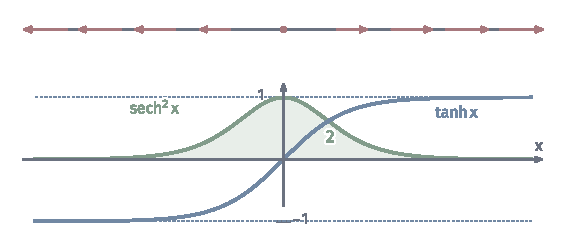
\includegraphics[width=96mm]{figures/04-spaces-measures-and-geometry/04-manifolds/matplotlib/mcalc-noncompact-flux/figure.pdf}
  \caption{$M=\mathbb R$上的$X=\tanh(x)\,\partial_x$。上方的红箭头是向量场本身，两端趋于$\pm\partial_x$。下方绿线是散度$\operatorname{sech}^2x$，浅绿面积为$2$；蓝线是$X$的分量$\tanh x$，它在两端趋于$\pm1$，这两个极限恰是逃向无穷远的流量。}
  \label{fig:mcalc-noncompact-flux}
\end{BookInlineFigure}

问题在于$fX$没有紧支撑。图~\ref{fig:mcalc-noncompact-flux}上方的箭头显示，流量一直流向无穷远，散度的累计$2$由这两股流量解释。非紧情形要使用分部积分，须验证紧支撑，或者验证被积函数衰减得足够快，使截断后边界项的极限为零。

\paragraph{弱导数与场方程的接口}
式~\eqref{eq:mcalc-integration-by-parts}对紧支撑的$f$不含边界项，可以反过来用作定义。第~\ref{chap:smoothing-weak-derivatives}章在欧氏开集上，用与紧支撑试验函数的积分关系定义弱导数。流形上同样可以说：局部可积的向量场$Y$是函数$u$的弱梯度，若对所有紧支撑于$M$内部的光滑向量场$X$，
\begin{equation}
\int_Mu\,\operatorname{div}X\,\mathrm dV_g=-\int_Mg(Y,X)\,\mathrm dV_g .
\label{eq:mcalc-weak-gradient}
\end{equation}
对光滑的$u$，$Y=\operatorname{grad}u$满足这一式；对不光滑的$u$，它在不求导的前提下刻画了“梯度”。

看圆周上的例子。取$S^1$的角度坐标$\theta\in(-\pi,\pi]$，度量$\mathrm d\theta^2$，$u(\theta)=\lvert\theta\rvert$。$u$在$\theta=0$与$\theta=\pm\pi$处有折点，不是$C^1$函数。对周期的光滑函数$X$，在$(-\pi,0)$与$(0,\pi)$上分别分部积分，
\[
\int_{-\pi}^{\pi}\lvert\theta\rvert X'\,\mathrm d\theta=\pi X(\pi)-\pi X(-\pi)-\int_0^\pi X\,\mathrm d\theta+\int_{-\pi}^0X\,\mathrm d\theta .
\]
边界项因$X$的周期性相消，于是$u$有弱梯度$Y=\operatorname{sgn}(\theta)\,\partial_\theta$。在$\theta=0$处，两侧的边界项因$u$连续而相消，所以折点不妨碍弱导数存在；若函数在某点跳跃，这样的项就消不掉，第~\ref{chap:smoothing-weak-derivatives}章已讨论过这种差别。

同理，方程$\Delta_gu=s$的弱形式是：对所有紧支撑的光滑$\varphi$，
\begin{equation}
-\int_Mg(\operatorname{grad}u,\operatorname{grad}\varphi)\,\mathrm dV_g=\int_Ms\varphi\,\mathrm dV_g ,
\label{eq:mcalc-weak-laplace}
\end{equation}
它只要求$u$有一阶弱导数。下一节的Sobolev空间为这些弱形式提供函数类，而弱解的存在、唯一与边值问题可参考\BookChapterRef{chap:elliptic-equations}{卷六第4章“椭圆方程与边值问题”}。

\section{流形上的函数空间}
\label{sec:mcalc-function-spaces}

上一节的弱梯度与弱形式需要一个函数类：函数本身可积到什么程度，弱导数可积到什么程度。欧氏区域上，这由$L^p$与Sobolev空间回答（第~\ref{chap:function-normed-spaces}章与第~\ref{chap:sobolev-spaces}章）。流形上没有全局坐标，但紧流形可以用有限张坐标图覆盖，每张图里都可以借用欧氏的结果。

本节说明怎样把这些空间搬到紧流形上，哪些性质能搬，搬的时候要核对什么。非紧流形放在最后讨论。

\paragraph{$L^p$空间}
第~\ref{sec:mcalc-function-integration}小节已经把黎曼体积做成$M$上的测度$\operatorname{vol}_g$。对$1\leq p<\infty$，定义
\begin{equation}
\lVert u\rVert_{L^p(M,g)}=\Bigl(\int_M\lvert u\rvert^p\,\mathrm dV_g\Bigr)^{1/p},
\label{eq:mcalc-lp-norm}
\end{equation}
$L^p(M,g)$是使其有限的可测函数（几乎处处相等者视为同一元素）组成的空间；$p=\infty$时取本性上确界。这是一般测度空间上的$L^p$空间的特例，所以第~\ref{chap:function-normed-spaces}章的结论直接适用：它是Banach空间，$p=2$时是Hilbert空间。可测向量场$Y$属于$L^p$，指函数$\lVert Y\rVert_g$属于$L^p(M,g)$，这样的向量场同样构成Banach空间。

\begin{theorem}[紧流形上$L^p$与度量的选择无关]
\label{thm:mcalc-lp-metric-independence}
设$M$是紧流形，$g$与$g'$是$M$上的两个黎曼度量，$1\leq p<\infty$。则存在常数$0<c\leq C$，使对所有可测函数$u$，
\begin{equation}
c\,\lVert u\rVert_{L^p(M,g)}\leq\lVert u\rVert_{L^p(M,g')}\leq C\,\lVert u\rVert_{L^p(M,g)}.
\label{eq:mcalc-lp-equivalence}
\end{equation}
因此$L^p(M,g)$与$L^p(M,g')$是同一个函数集合，范数等价。
\end{theorem}

\begin{proof}
在任一坐标图中令$\kappa=\sqrt{\det\bm G'}/\sqrt{\det\bm G}$。由式~\eqref{eq:mcalc-density-change}，换图时分子分母都乘以$\lvert\det\bm A\rvert$，所以$\kappa$是$M$上与坐标无关的函数，并且连续、处处为正，满足$\mathrm dV_{g'}=\kappa\,\mathrm dV_g$。

紧集上的正连续函数有正的最小值$m$和有限的最大值$m'$，于是
\[
m\int\lvert u\rvert^p\,\mathrm dV_g\leq\int\lvert u\rvert^p\,\mathrm dV_{g'}\leq m'\int\lvert u\rvert^p\,\mathrm dV_g .
\]
开$p$次方即得，$c=m^{1/p}$，$C=m'^{1/p}$。
\end{proof}

所以在紧流形上，“$u$属于$L^p$”是一个不依赖度量的性质，度量只影响范数的具体数值。球面的半径变化是这个定理的最简单情形：半径$a$的球面上$\mathrm dV=a^2\,\mathrm dV_{S^2}$，常数$c=C=a^{2/p}$。

\paragraph{Sobolev空间的内在定义}
有了第~\ref{sec:mcalc-integration-by-parts}节的弱梯度，一阶Sobolev空间可以不借坐标定义。设$M$是紧流形（暂设无边界），$1\leq p<\infty$。若$u\in L^p(M,g)$存在弱梯度$Y$且$Y$属于$L^p$，称$u\in W^{1,p}(M)$，记$\operatorname{grad}u=Y$，并取范数
\begin{equation}
\lVert u\rVert_{W^{1,p}}=\Bigl(\lVert u\rVert_{L^p}^p+\bigl\lVert\,\lVert\operatorname{grad}u\rVert_g\bigr\rVert_{L^p}^p\Bigr)^{1/p}.
\label{eq:mcalc-sobolev-norm}
\end{equation}

弱梯度若存在则几乎处处唯一：两个弱梯度之差$Z$满足$\int g(Z,X)\,\mathrm dV_g=0$对所有光滑$X$成立，在每张坐标图中用光滑向量场逼近$Z$的截断，即得$Z=0$几乎处处，这与第~\ref{chap:smoothing-weak-derivatives}章中弱导数唯一性的论证相同。

前面$S^1$上的$u=\lvert\theta\rvert$就在这个空间里。它的弱梯度是$\operatorname{sgn}(\theta)\,\partial_\theta$，其度量长度恒为$1$。对比圆周上的光滑函数$u_0=1+\tfrac12\cos\theta$，它的$W^{1,2}$范数可以直接计算：
\[
\lVert u_0\rVert_{L^2}^2=\int_0^{2\pi}\bigl(1+\tfrac12\cos\theta\bigr)^2\,\mathrm d\theta=\frac94\pi ,\qquad
\lVert u_0'\rVert_{L^2}^2=\frac\pi4 .
\]
两者相加，$\lVert u_0\rVert_{W^{1,2}}^2=\tfrac52\pi$。这里用的是$S^1$的标准度量；下面的定理说明这个空间在选取度量之后的性质。

\begin{theorem}[$W^{1,p}(M)$的完备性]
\label{thm:mcalc-sobolev-complete}
在紧黎曼流形上，$W^{1,p}(M)$是Banach空间。
\end{theorem}

\begin{proof}
设$(u_m)$是$W^{1,p}$中的Cauchy列，则$(u_m)$与$(\operatorname{grad}u_m)$分别是$L^p$函数与$L^p$向量场中的Cauchy列。由$L^p$的完备性，$u_m\to u$，$\operatorname{grad}u_m\to Y$。

对任一光滑向量场$X$，$\operatorname{div}X$与$\lVert X\rVert_g$在紧集$M$上有界，由Hölder不等式，式~\eqref{eq:mcalc-weak-gradient}两端可以取极限：
\[
\begin{aligned}
\int u\,\operatorname{div}X\,\mathrm dV_g&=\lim_m\int u_m\operatorname{div}X\,\mathrm dV_g\\
&=-\lim_m\int g(\operatorname{grad}u_m,X)\,\mathrm dV_g=-\int g(Y,X)\,\mathrm dV_g .
\end{aligned}
\]
所以$Y$是$u$的弱梯度，$u\in W^{1,p}$，并且$u_m\to u$在$W^{1,p}$范数下成立。
\end{proof}

\paragraph{坐标图中的定义与等价性}
内在定义便于理解，计算与证明则常常借助坐标。取有限个坐标图$(U_\alpha,\varphi_\alpha)$，$\alpha=1,\ldots,m$，覆盖$M$，并要求每个$\overline{U_\alpha}$紧，且落在一张更大的坐标图内；紧性保证这样的有限覆盖存在。再取从属的单位分解$\{\psi_\alpha\}$。

对函数$u$，$(\psi_\alpha u)\circ\varphi_\alpha^{-1}$是$\mathbb R^n$上紧支撑的函数，令
\begin{equation}
\lVert u\rVert'_{W^{1,p}}=\sum_{\alpha=1}^m\bigl\lVert(\psi_\alpha u)\circ\varphi_\alpha^{-1}\bigr\rVert_{W^{1,p}(\mathbb R^n)} .
\label{eq:mcalc-chart-sobolev}
\end{equation}
图~\ref{fig:mcalc-chart-cover}在圆周上演示了这个构造：单位分解把$u$切成两段，每段落在一张图的内部，可以在普通的区间上用Sobolev范数度量。

\begin{BookInlineFigure}
  \centering
  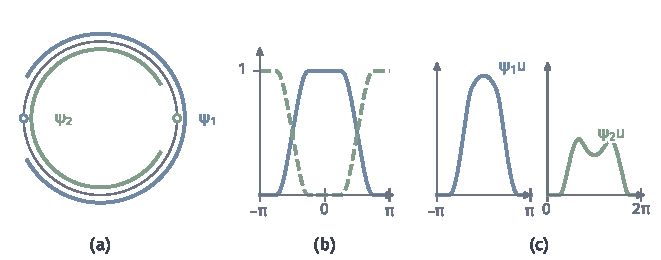
\includegraphics[width=112mm]{figures/04-spaces-measures-and-geometry/04-manifolds/matplotlib/mcalc-chart-cover/figure.pdf}
  \caption{圆周上的有限覆盖与单位分解。(a)两张角度图，分别漏掉$(-1,0)$与$(1,0)$（空心圆），蓝弧与绿弧是$\psi_1,\psi_2$的支撑，每个支撑严格落在所在的图内。(b)$\psi_1$（实线）与$\psi_2=1-\psi_1$（虚线），横轴是角度$\theta$。(c)$u=1+\tfrac12\cos\theta$被切成的两段$\psi_1u$与$\psi_2u$，分别画在各自的图中，都是区间上紧支撑的函数。}
  \label{fig:mcalc-chart-cover}
\end{BookInlineFigure}

在每个$\overline{U_\alpha}$上，度量矩阵的特征值有正的上下界，所以$\lVert\xi\rVert_g$与坐标欧氏长度$\lVert\xi\rVert_2$、$\mathrm dV_g$与$\mathrm d\bm x$在常数倍内可比。单位分解函数及其导数有界，并且乘积规则对弱梯度仍成立：
\[
\operatorname{grad}(\psi_\alpha u)=\psi_\alpha\operatorname{grad}u+u\operatorname{grad}\psi_\alpha .
\]

由这些估计可以得到$\lVert\cdot\rVert'$与$\lVert\cdot\rVert_{W^{1,p}}$等价，并且换用另一组有限覆盖或单位分解只改变等价常数。完整写出常数需要把上面的上下界逐项收集，篇幅较长；结论的含义是，一阶Sobolev空间作为函数集合只取决于光滑结构，度量与覆盖的选择只影响范数的数值。

这一等价性是搬运欧氏结论的通道。例如光滑函数的稠密性：对$u\in W^{1,p}(M)$，把每个$(\psi_\alpha u)\circ\varphi_\alpha^{-1}$用第~\ref{chap:smoothing-weak-derivatives}章的磨光逼近，再拉回求和，得到逼近$u$的光滑函数。磨光后支撑仍落在稍大的坐标域内，这正是要求$\overline{U_\alpha}$落在更大坐标图中的原因。

高阶空间$W^{k,p}(M)$可以同样用坐标图定义，也可以用协变导数$\nabla^ku$内在地定义，两者在紧流形上等价，证明需要逐阶比较协变导数与坐标偏导数，读者可查阅几何分析方面的教材。第~\ref{chap:sobolev-spaces}章的连续嵌入与紧嵌入也可以经有限覆盖搬到紧流形上，所得常数依赖覆盖与度量。

\paragraph{带边界的情形}
紧的带边界流形上，边界附近的坐标图取值于半空间。第~\ref{chap:sobolev-spaces}章在半空间或光滑边界区域上建立的延拓、迹与约束子空间，经边界坐标图搬到流形上，须逐项核对两件事。

一是所用的欧氏结论是否要求边界光滑：流形的边界在定义上光滑，但带角点的区域不在这一框架内。二是结论在坐标变换下是否保持：例如“迹为零”的子空间与坐标无关，而迹的具体范数依赖坐标与度量。Dirichlet条件对应$W^{1,p}$中“迹为零”的闭子空间，Neumann条件则不进入空间的定义，而是在弱形式中由边界项自然体现。

\paragraph{非紧流形}
非紧流形上，有限覆盖不复存在，逐图的控制与整体范数有限是两回事。$\mathbb R$上的常函数$u\equiv1$在每个有界坐标区间上都属于$L^p$与$W^{1,p}$，整体上却不属于$L^p(\mathbb R)$。为区分这两层，记$L^p_{\mathrm{loc}}$与$W^{1,p}_{\mathrm{loc}}$为在每个紧子集上满足相应条件的函数。局部空间不依赖度量，整体空间则依赖度量。

整体空间对度量的依赖在非紧时不再是范数等价那么简单。$\mathbb R$上取$g=\mathrm dx^2$与$g'=(1+x^2)^2\mathrm dx^2$，二者的体积密度之比为$1+x^2$，无界。函数$u(x)=(1+\lvert x\rvert)^{-1}$满足
\[
\int_{\mathbb R}u^2\,\mathrm dx<\infty,\qquad\int_{\mathbb R}u^2(1+x^2)\,\mathrm dx=\infty ,
\]
第二个积分发散是因为被积函数在无穷远处趋于$1$。所以$u\in L^2(\mathbb R,g)$却$u\notin L^2(\mathbb R,g')$，两个空间是不同的集合。

欧氏结论也不能无条件继承。紧流形上$W^{1,2}(M)\hookrightarrow L^2(M)$是紧嵌入；$\mathbb R$上则不然。取支撑含于$(0,1)$的非零光滑函数$\varphi$及其平移$\varphi(x-k)$，$k=1,2,\ldots$，它们在$W^{1,2}(\mathbb R)$中有界，而由于支撑不交，
\[
\lVert\varphi(\cdot-k)-\varphi(\cdot-l)\rVert_{L^2}=\sqrt2\,\lVert\varphi\rVert_{L^2},\qquad k\neq l ,
\]
所以这列函数没有$L^2$收敛的子列。这与第~\ref{chap:functions-as-vectors}章中无限维闭球不紧的现象同源：平移把一个固定的函数送到互不相交的位置，相当于在$L^2$中给出无穷多个互相正交的方向。

非紧流形上嵌入不等式的常数还可能因体积或曲率失去一致的控制而失效，使用时须先核对流形的整体几何条件。

\section{本章小结}
\label{sec:mcalc-summary}

本章开头的问题是：在流形上怎样求导、怎样积分，内部的变化怎样汇总到边界。第一部分只用光滑结构回答。微分形式是对多个切向量的交替读数，楔积按次数满足交换符号规则，拉回沿映射反向作用且对任何光滑映射都有定义，外微分把$k$形式变为$k+1$形式，对函数就是$\mathrm df$，与楔积、拉回相容，并满足$\mathrm d\circ\mathrm d=0$。闭而不恰当的形式，如穿孔平面上的$(x_1\,\mathrm dx_2-x_2\,\mathrm dx_1)/r^2$，反映流形的拓扑。

积分最高次形式还需要定向：形式的系数按带符号的Jacobian行列式变换，只有在定向图册中它才与积分换元公式中的绝对值一致。球面的两张球极投影图要调整一个坐标的符号才构成定向图册，M\"obius带则根本没有定向。边界的诱导定向采用“外法向在前”的约定，在这一约定下，Stokes公式把$\mathrm d\omega$在流形上的积分与$\omega$在边界上的积分联系起来，对紧支撑的$(n-1)$形式成立，紧支撑与定向都不可省略；Green、Gauss与经典Stokes公式是它在平面区域、三维区域与有向曲面上的特例。

第二部分加入黎曼度量。体积密度$\sqrt{\det\bm G}\,\mathrm d\bm x$以Jacobian的绝对值变换，因而不需要定向，在可定向时对应体积形式。由它得到的函数积分是一个测度积分，与定向无关，随度量改变，也不同于样本的采样测度。梯度用度量把$\mathrm df$变成向量，Hessian用Levi-Civita联络扣除方向场的变化，是对称双线性型；散度是协变导数的迹，坐标式只含体积密度；Laplace--Beltrami算子是梯度的散度，在本书约定下非正。球面高度函数把这些运算串在一起：$\operatorname{grad}h$沿经线指向北极，$\operatorname{Hess}h=-hg$，$\Delta h=-2h$，三个结果彼此印证。

梯度、散度与散度定理合成分部积分公式，边界项在闭流形、紧支撑或Dirichlet、Neumann条件下消失，非紧时须另行核对；它也给出弱梯度与场方程弱形式的定义。在紧流形上，有限坐标覆盖、单位分解和黎曼体积把$L^p$与Sobolev空间搬了过来，空间本身不依赖度量的选择，完备性与稠密性得以保留。非紧时须区分局部与整体的控制，欧氏的紧嵌入等结论不能无条件继承。这些运算为后续的流形优化与场方程提供了合法使用的条件。

